% Copyright (C) 2010,2011,2012,2013,2014,2015,2016 The ESPResSo project
% Copyright (C) 2002,2003,2004,2005,2006,2007,2008,2009,2010 
%   Max-Planck-Institute for Polymer Research, Theory Group
%  
% This file is part of ESPResSo.
%   
% ESPResSo is free software: you can redistribute it and/or modify it
% under the terms of the GNU General Public License as published by the
% Free Software Foundation, either version 3 of the License, or (at your
% option) any later version.
%  
% ESPResSo is distributed in the hope that it will be useful, but
% WITHOUT ANY WARRANTY; without even the implied warranty of
% MERCHANTABILITY or FITNESS FOR A PARTICULAR PURPOSE.  See the GNU
% General Public License for more details.
%  
% You should have received a copy of the GNU General Public License
% along with this program.  If not, see <http://www.gnu.org/licenses/>.
%
\documentclass[
a4paper,                        % paper size
11pt,                           % font size
twoside,                        % two sided
footsepline,                    % add a line to separate the footer
headsepline,                    % add a line to separate the header
headexclude,                    % header does not belong to the text
footexclude,                    % footer does not belong to the text
pagesize,                       % set the pagesize in a DVI document
]{scrartcl}

% Copyright (C) 2010,2011,2012 The ESPResSo project
% Copyright (C) 2002,2003,2004,2005,2006,2007,2008,2009,2010
%  Max-Planck-Institute for Polymer Research, Theory Group
%  
% This file is part of ESPResSo.
%   
% ESPResSo is free software: you can redistribute it and/or modify it
% under the terms of the GNU General Public License as published by the
% Free Software Foundation, either version 3 of the License, or (at your
% option) any later version.
%  
% ESPResSo is distributed in the hope that it will be useful, but
% WITHOUT ANY WARRANTY; without even the implied warranty of
% MERCHANTABILITY or FITNESS FOR A PARTICULAR PURPOSE.  See the GNU
% General Public License for more details.
%  
% You should have received a copy of the GNU General Public License
% along with this program.  If not, see <http://www.gnu.org/licenses/>.
%
\usepackage[draft]{varioref}    % defines \vref
\usepackage{hyperref}           % automatically creates links when
                                % using pdflatex, defines \url
\usepackage{ifpdf}              % defines \ifpdf
\usepackage{graphicx}           % handles graphics
\usepackage{color}              % use colors

\usepackage{amsmath}

\usepackage{verbatim}           % required for \verbatim and \endverbatim
\usepackage{fancyvrb}
\usepackage{calc}               % compute length
\usepackage{ifthen}             % provide ifthen
\usepackage{xspace}
\usepackage{units}
\usepackage[numbers]{natbib}

% For building the distribution docs, disable todo boxes.
%\usepackage[disable]{todonotes}
\usepackage{todonotes}

\newcommand{\es}{\mbox{\textsf{ESPResSo}}\xspace}
\newcommand{\ie}{\textit{i.e.}\xspace}
\newcommand{\eg}{\textit{e.g.}\xspace}
\newcommand{\etal}{\textit{et al.}\xspace}

\newcommand{\codebox}[1]%
{\texttt{#1}}

\DefineVerbatimEnvironment{code}{Verbatim}%
{commandchars=\\\{\}}
\makeatletter
\newenvironment{tclcode}
{%
  \addtolength{\linewidth}{-2em}% set the line length
  \@minipagetrue%%%DPC%%%
  \@tempswatrue%%%DPC%%%
  \hsize=\linewidth%
  \setbox0=\vbox\bgroup\verbatim
}{\endverbatim
  \unskip\setbox0=\lastbox%%%DPC%%%
  \egroup
  \par%
  \noindent\hspace{1em}%
  \codebox{\box0}%
  \par\noindent%
}
\makeatother

% \newcommand{\todo}[1]{
%   \marginpar{%
%     \setlength{\fboxrule}{1pt}
%     \fcolorbox{red}{yellow}{%
%       \parbox{\marginparwidth-2\fboxrule-2\fboxsep}{%
%         \bf\raggedright\scriptsize #1%
%       }%
%     }%
%   }%
% }

\makeatletter
\renewcommand{\minisec}[1]{\@afterindentfalse \vskip 1.5ex
  {\parindent \z@
    \raggedsection\normalfont\sffamily\itshape\nobreak#1\par\nobreak}%
  \@afterheading}
\makeatother

\newcommand{\esptitlehead}{
  \titlehead{
    \begin{center}
      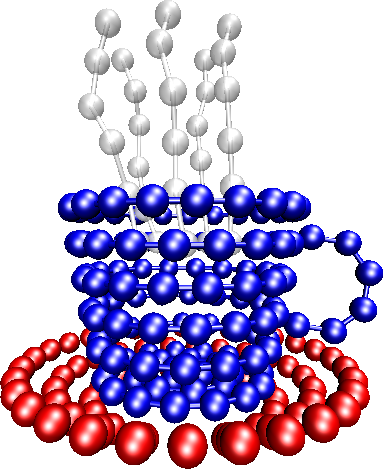
\includegraphics[width=5cm]{logo/transparentbg}
    \end{center}
  }
}


\begin{document}
\esptitlehead
\title{Tutorial 2: A simple charged system%
\ifdefined\esversion%
\thanks{For \es \esversion}%
\fi%
}

\maketitle
\tableofcontents

\section{Introduction}

This tutorial introduces some of the basic features of \es\ for charged systems
by constructing a simulation script for a simple salt crystal. We assume that
the reader is familiar with the basic concepts of Python and MD simulations. The
code pieces can be copied step by step into a python script file, which then can
be run using \verb|pypresso <file>| from the \es build directory.

\section{Basic set up}

We start with setting up all the relevant simulation parameters in one place:

\begin{python}
# System parameters
n_part = 200
n_ionpairs = n_part/2
density = 0.7
time_step = 0.01
temp = 1.0
gamma = 1.0
l_bjerrum = 1.0

num_steps_equilibration = 1000
num_configs = 100
integ_steps_per_config = 1000

# Particle parameters
types       = {"Anion":          0, "Cation": 1}
numbers     = {"Anion": n_ionpairs, "Cation": n_ionpairs}
charges     = {"Anion":       -1.0, "Cation": 1.0}
lj_sigmas   = {"Anion":        1.0, "Cation": 1.0}
lj_epsilons = {"Anion":        1.0, "Cation": 1.0}

WCA_cut = 2.**(1. / 6.)
lj_cuts     = {"Anion":  WCA_cut * lj_sigmas["Anion"], 
               "Cation": WCA_cut * lj_sigmas["Cation"]}
\end{python}

These variables do not change anything in the simulation engine, but
are just standard Python variables. They are used to increase the
readability and flexibility of the script. The box length is not a
parameter of this simulation, it is calculated from the number of
particles and the system density. This allows to change the parameters
later easily, e.~g.\ to simulate a bigger system.
We use dictionaries for all particle related parameters, which is less error-prone and
readable as we will see later when we actually need the values. The parameters here define a purely repulsive, 
equally sized, monovalent salt.

The simulation engine itself is modified by changing the
espressomd.System() properties. We create an instance \emph{system} and
set the box length, periodicity and time step. The skin depth \verb|skin| 
is a parameter for the link--cell system which tunes its
performance, but shall not be discussed here. Further, we activate the langevin thermostat
for our NVT ensemble with temperature \verb|temp| and friction coefficient \verb|gamma|. 


\begin{python}
# Setup System
system = espressomd.System()
box_l = (n_part / density)**(1. / 3.)
system.box_l = [box_l, box_l, box_l]
system.periodicity = [1, 1, 1]
system.time_step = time_step
system.cell_system.skin = 0.3
system.thermostat.set_langevin(kT=temp, gamma=gamma)
\end{python}

We now fill this simulation box with particles at random positions, using type and charge from our dictionaries.
Using the length of the particle list \emph{system.part} for the id, we make sure that our particles are numbered consecutively.
The particle type is used to link non-bonded interactions to a certain group of particles.

\begin{python}
# Place particles
for i in range(n_ionpairs):
    system.part.add(
            id=len(system.part), 
            type=types["Anion"],  
            pos=numpy.random.random(3) * box_l, 
            q=charges["Anion"])
for i in range(n_ionpairs):
    system.part.add(
            id=len(system.part), 
            type=types["Cation"], 
            pos=numpy.random.random(3) * box_l, 
            q=charges["Cation"])
\end{python}

Before we can really start the simulation, we have to specify the
interactions between our particles. We already defined the Lennard-Jones parameters at the beginning,
what is left is to specify the combination rule and to iterate over particle type pairs. For simplicity, 
we implement only the \emph{Lorentz-Berthelot} rules. 
We pass our interaction pair to \verb|system.non_bonded_inter[*,*]| and set the 
pre-calculated LJ parameters \emph{epsilon}, \emph{sigma} and \emph{cutoff}. With \verb|shift="auto"|,
we shift the interaction potential to the cutoff so that $U_{LJ}(r_{cutoff})=0$.

\begin{python}
def combination_rule_epsilon(rule, eps1, eps2):
    if rule=="Lorentz":
        return (eps1*eps2)**0.5
    else:
        return ValueError("No combination rule defined")

def combination_rule_sigma(rule, sig1, sig2):
    if rule=="Berthelot":
        return (sig1+sig2)*0.5
    else:
        return ValueError("No combination rule defined")

# Lennard-Jones interactions parameters 
for s in [["Anion", "Cation"], 
          ["Anion", "Anion"], 
          ["Cation", "Cation"]]:
        lj_sig = combination_rule_sigma(
                "Berthelot",
                lj_sigmas[s[0]],lj_sigmas[s[1]])
        lj_cut = combination_rule_sigma(
                "Berthelot",
                lj_cuts[s[0]],lj_cuts[s[1]])
        lj_eps = combination_rule_epsilon(
                "Lorentz",
                lj_epsilons[s[0]],lj_epsilons[s[1]])

        system.non_bonded_inter[types[s[0]], types[s[1]]].\
            lennard_jones.set_params(
            epsilon=lj_eps,
            sigma=lj_sig,
            cutoff=lj_cut,
            shift="auto")

\end{python}

\newpage

\section{Equilibration}

With randomly positioned particles, we most likely have huge overlap and the strong repulsion will
cause the simulation to crash. The next step in our script therefore is a suitable LJ equilibration.
This is known to be a tricky part of a simulation and several approaches exist to reduce the particle overlap.
Here, we use a highly damped system (huge gamma in the thermostat) and cap the forces of the LJ interaction.
We use \verb|system.analysis.mindist| to get the minimal distance between all particles pairs. This value
is used to progessively increase the force capping. This results in a slow increase of the force capping at
strong overlap. At the end, we reset our thermostat to the target values and deactivate the force cap by setting 
it to zero.

\begin{python}
print("\n--->Lennard Jones Equilibration")
max_sigma = max(lj_sigmas.values())
min_dist = 0.0
cap = 10.0
#Warmup Helper: Cold, highly damped system
system.thermostat.set_langevin(kT=temp*0.1, gamma=gamma*50.0)

while min_dist < max_sigma:
    #Warmup Helper: Cap max. force, increase slowly for overlapping particles
    min_dist = system.analysis.mindist(
            [types["Anion"],types["Cation"]],
            [types["Anion"],types["Cation"]])
    cap += min_dist
    system.non_bonded_inter.set_force_cap(cap)
    system.integrator.run(10)

#Don't forget to reset thermostat and force cap
system.thermostat.set_langevin(kT=temp, gamma=gamma)
system.non_bonded_inter.set_force_cap(0)
\end{python}

\es\ uses so-called \emph{actors} for electrostatics, magnetostatics and
hydrodynamics. This ensures that unphysical combinations of algorithms are
avoided, for example simultaneous usage of two electrostatic interactions.
Adding an actor to the system also activates the method and calls necessary
initialization routines. Here, we define a P$^3$M object with paramters Bjerrum
length and rms force errow . This automatically starts a
tuning function which tries to find optimal parameters for P$^3$M and prints them
to the screen:

\newpage

\begin{python}
print("\n--->Tuning Electrostatics")
p3m = electrostatics.P3M(bjerrum_length=l_bjerrum, accuracy=1e-3)
system.actors.add(p3m)
\end{python}

Before the production part of the simulation, we do a quick temperature 
equilibration. For the output, we gather all energies with
\verb|system.analysis.energy()|, calculate the temperature from the ideal part and 
print it to the screen along with the total and coulombic energies.
We integrate for a certain amount of steps with \verb|system.integrator.run(100)|.



\begin{python}
print("\n--->Temperature Equilibration")
system.time = 0.0
for i in range(num_steps_equilibration/100):
    energy = system.analysis.energy()
    temp_measured = energy['ideal'] / ((3.0 / 2.0) * n_part)
    print("t={0:.1f}, E_total={1:.2f}, E_coulomb={2:.2f}, T={3:.4f}".\
            format(system.time, energy['total'], 
                   energy['coulomb'], temp_measured))
    system.integrator.run(100)
\end{python}

\section{Running the simulation}

Now we can integrate the particle trajectories for a couple of time
steps. Our integration loop basically looks like the equilibration:

\begin{python}
print("\n--->Integration")
system.time = 0.0
for i in range(num_configs):
    energy = system.analysis.energy()
    temp_measured = energy['ideal'] / ((3.0 / 2.0) * n_part)
    print("t={0:.1f}, E_total={1:.2f}, E_coulomb={2:.2f}, T={3:.4f}".\
            format(system.time, energy['total'],
                   energy['coulomb'], temp_measured))
    system.integrator.run(integ_steps_per_config)

    # Interally append particle configuration
    system.analysis.append()
\end{python}

Additionally, we append all particle configurations in the core with \verb|system.analysis.append()| for
a very convenient analysis later on. 

\begin{figure}[tb]
  \centering
  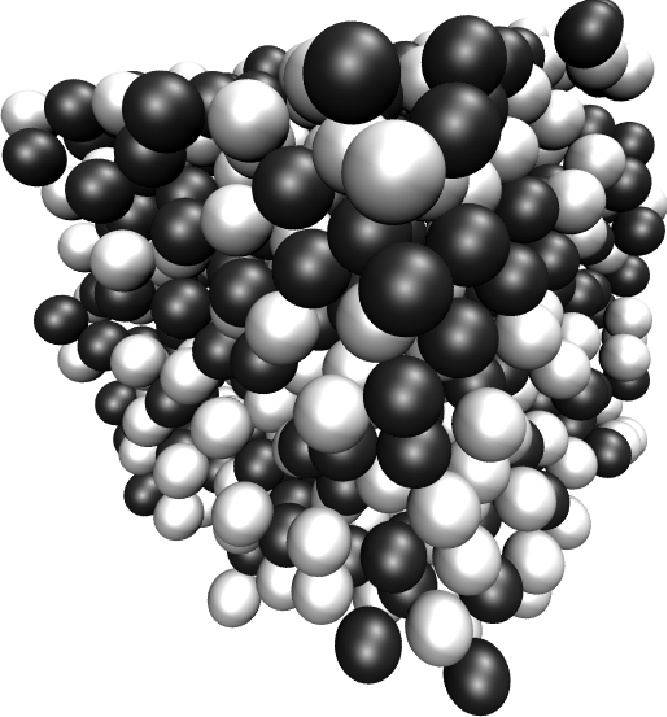
\includegraphics[width=0.3\textwidth]{figures/salt}
  \caption{VMD Snapshot of the salt system}
  \label{fig:snapshot}
\end{figure}

\section{Analysis}

Now, we want to calculate the averaged radial distribution functions
$g_{++}(r)$ and $g_{+-}(r)$ with the \verb|rdf()| command from \verb|system.analysis|: 

\begin{python}
print("\n--->Analysis")
# Calculate the averaged rdfs
rdf_bins = 100
r_min  = 0.0
r_max  = system.box_l[0]/2.0
r,rdf_00 = system.analysis.rdf(rdf_type='<rdf>', 
                            type_list_a=[types["Anion"]],
                            type_list_b=[types["Anion"]], 
                            r_min=r_min,
                            r_max=r_max, 
                            r_bins=rdf_bins)
r,rdf_01 = system.analysis.rdf(rdf_type='<rdf>', 
                            type_list_a=[types["Anion"]],
                            type_list_b=[types["Cation"]], 
                            r_min=r_min,
                            r_max=r_max, 
                            r_bins=rdf_bins)

\end{python}

The shown \verb|rdf()| commands return the radial distribution functions for
equally and oppositely charged particles for specified radii and number of bins. 
In this case, we calulate the averaged rdf of the the stored
configurations, denoted by the chevrons in \verb|rdf_type='<rdf>'|. Using
\verb|rdf_type='rdf'| would simply calculate the rdf of the current particle
configuration. The results are two numpy arrays containing the $r$ and $g(r)$
values. Finally we write the data into a file with standard python output routines.

\begin{python}
rdf_fp = open('rdf.data', 'w')
for i in range(rdf_bins):
    rdf_fp.write("%1.5e %1.5e %1.5e\n" % (r[i], rdf_00[i], rdf_01[i]))
rdf_fp.close()
print("\n--->Written rdf.data\n--->Done")
\end{python}

\begin{figure}[tb]
  \centering
  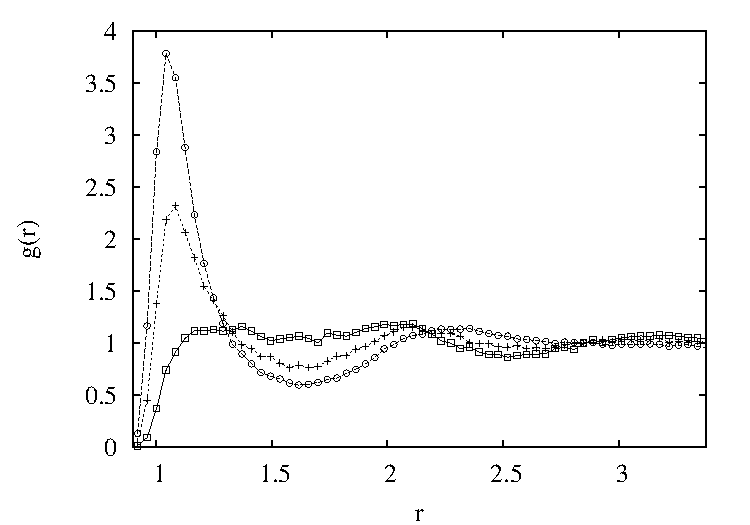
\includegraphics[width=0.6\textwidth]{figures/nacl-rdf}
  \caption{Radial distribution functions $g_{++}(r)$ between equal
    charges (rectangles) and $g_{+-}(r)$ for opposite charges
    (circles). The plus symbols denote $g(r)$ for an uncharged
    system.}
  \label{fig:rdf}
\end{figure}

Fig.~\ref{fig:rdf} shows the resulting radial distribution functions. In
addition, the distribution for a neutral system is given, which can be obtained
from our simulation script by simply not adding the P$^3$M actor to the system.
To view your own results, run \verb|gnuplot| in a Terminal window
and plot the simulation data:

\begin{python}
p 'rdf.data' u 1:2 w lp t 'g(r) ++' , '' u 1:3 w lp t 'g(r) +-'
\end{python}

\section{Task - Real units}

So far, the system has arbitrary units and is not connected to any real physical system.
Simulate a proper NaCl crystal with the force field parameter taken from:\\
\\
\noindent R. Fuentes-Azcatl and M. Barbosa, \emph{Sodium Chloride, NaCl/$\epsilon$ : New Force Field},\\ J. Phys. Chem. B, 2016, 120(9), pp 2460-2470
\begin{table}[h]
    \centering
    \begin{tabular}{l|llll}
           & $q/\mathrm{e}$  & $\sigma / \mathrm{\AA} $ & $(\epsilon /\mathrm{k_B})/\mathrm{K}$ & $m/\mathrm{u}$  \\
        \hline
        Na & +1     & 2.52          & 17.44                 & 22.99  \\
        \hline
        Cl & -1     & 3.85          & 192.45                & 35.453 
    \end{tabular}
\end{table}

Use the following system parameters:

\begin{table}[h]
    \centering
    \begin{tabular}{l|l}
        Temperature            & $298 \ \mathrm{K}$          \\
        \hline
        Friction Coeff.        & $5 \ \mathrm{ps^{-1}}$      \\
        \hline
        Density                & $1.5736 \ \mathrm{u}\mathrm{\AA^{-3}}$ \\
        \hline
        Bjerrum length($298 \ \mathrm{K}$) & $439.2 \ \mathrm{\AA}$      \\
        \hline
        Time step              & $2 \ \mathrm{fs}$
    \end{tabular}
\end{table}

To make your life more easy, don't try to equilibrate randomly positioned particles,
but set them up in a crystal structure close to equilibrium. If you do it right,
you don't even need the Lennard-Jones equilibration. 
To speed things up, don't go further than 1000 particles and use a P$^3$M accuracy of $10^{-2}$.
Your RDF should look like the plot in figure \ref{fig:nacl_units}.

\begin{figure}[h]
  \centering
  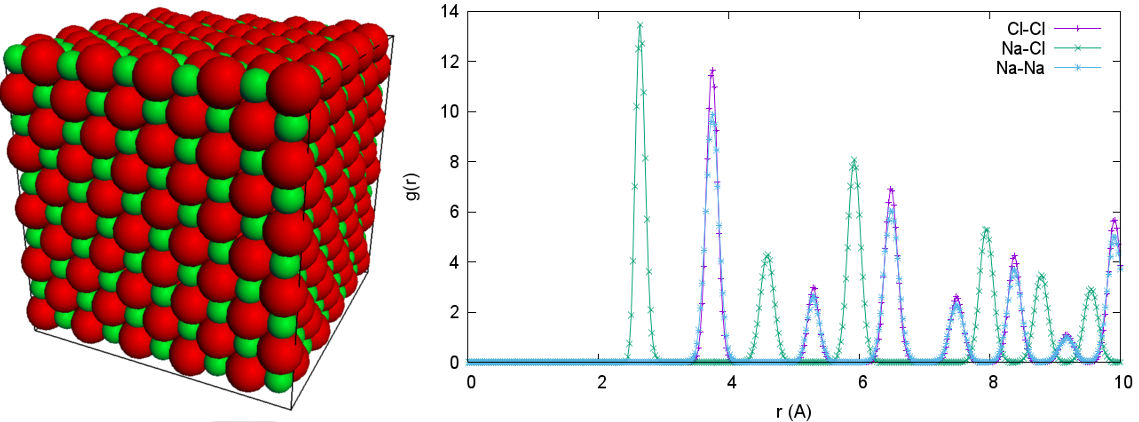
\includegraphics[width=0.9\textwidth]{figures/nacl_units.jpg}
  \caption{Snapshot and RDF of the parametrized NaCl crystal.}
  \label{fig:nacl_units}
\end{figure}

\end{document}
